
From \cite{dohu}. In order to illustrate the behavior of selected mixed finite elements in the solution 
of stationary Stokes flow,  we consider a two-dimensional problem 
in the square domain $\Omega=[0,1]\times[0,1]$, which possesses a closed-form analytical 
solution. The problem consists of determining the velocity field ${\bm v} = (u,v)$ and the 
pressure $p$ such that 
\[
-\nu \Delta {\bm v} + {\bm \nabla} p = {\bm b}  \quad\quad {\rm in} \; \Omega
\]
\[
{\bm \nabla} \cdot {\bm v} = 0 \quad\quad {\rm in} \; \Omega
\]
\[
{\bm v}={\bm 0} \quad\quad {\rm on} \; \Gamma
\]
where the fluid viscosity is taken as $\nu=1$. The components of the body force ${\bm b}$ are prescribed as 
\begin{eqnarray}
b_x &=& (12 - 24y) x^4 + (-24 + 48y) x^3 + (-48y + 72y^2 - 48 y^3 + 12) x^2 \nonumber\\
    && + (-2 + 24y -72y^2+48y^3)x + 1-4y + 12y^2-8y^3 \nonumber\\ 
b_y &=& (8 - 48y + 48 y^2) x^3 + (-12 + 72y - 72y^2) x^2  \nonumber\\
    && + (4 - 24y + 48y^2 - 48y^3 + 24y^4) x - 12y^2 + 24y^3 - 12y^4  \nonumber
\end{eqnarray}
With this prescribed body force, the exact solution is 
\begin{eqnarray}
u(x,y) &=& x^2(1- x)^2 (2y - 6y^2 + 4y^3)  \nonumber\\
v(x,y) &=& -y^2 (1 - y)^2 (2x - 6x^2 + 4x^3) \nonumber\\
p(x,y) &=& x(1 -x)- 1/6 \nonumber 
\end{eqnarray}
Note that the pressure obeys $\int_{\Omega} p \; d\Omega = 0$

\fbox{
\parbox{10cm}{{\bf features}
\begin{itemize}
\item $Q_1\times P_0$ element \index{$Q_1 \times P_0$}
\item incompressible flow
\item penalty formulation \index{penalty formulation}
\item Dirichlet boundary conditions (no-slip)
\item direct solver 
\item isothermal \index{isothermal}
\item isoviscous \index{isoviscous}
\item analytical solution \index{analytical solution}
\end{itemize}
}}

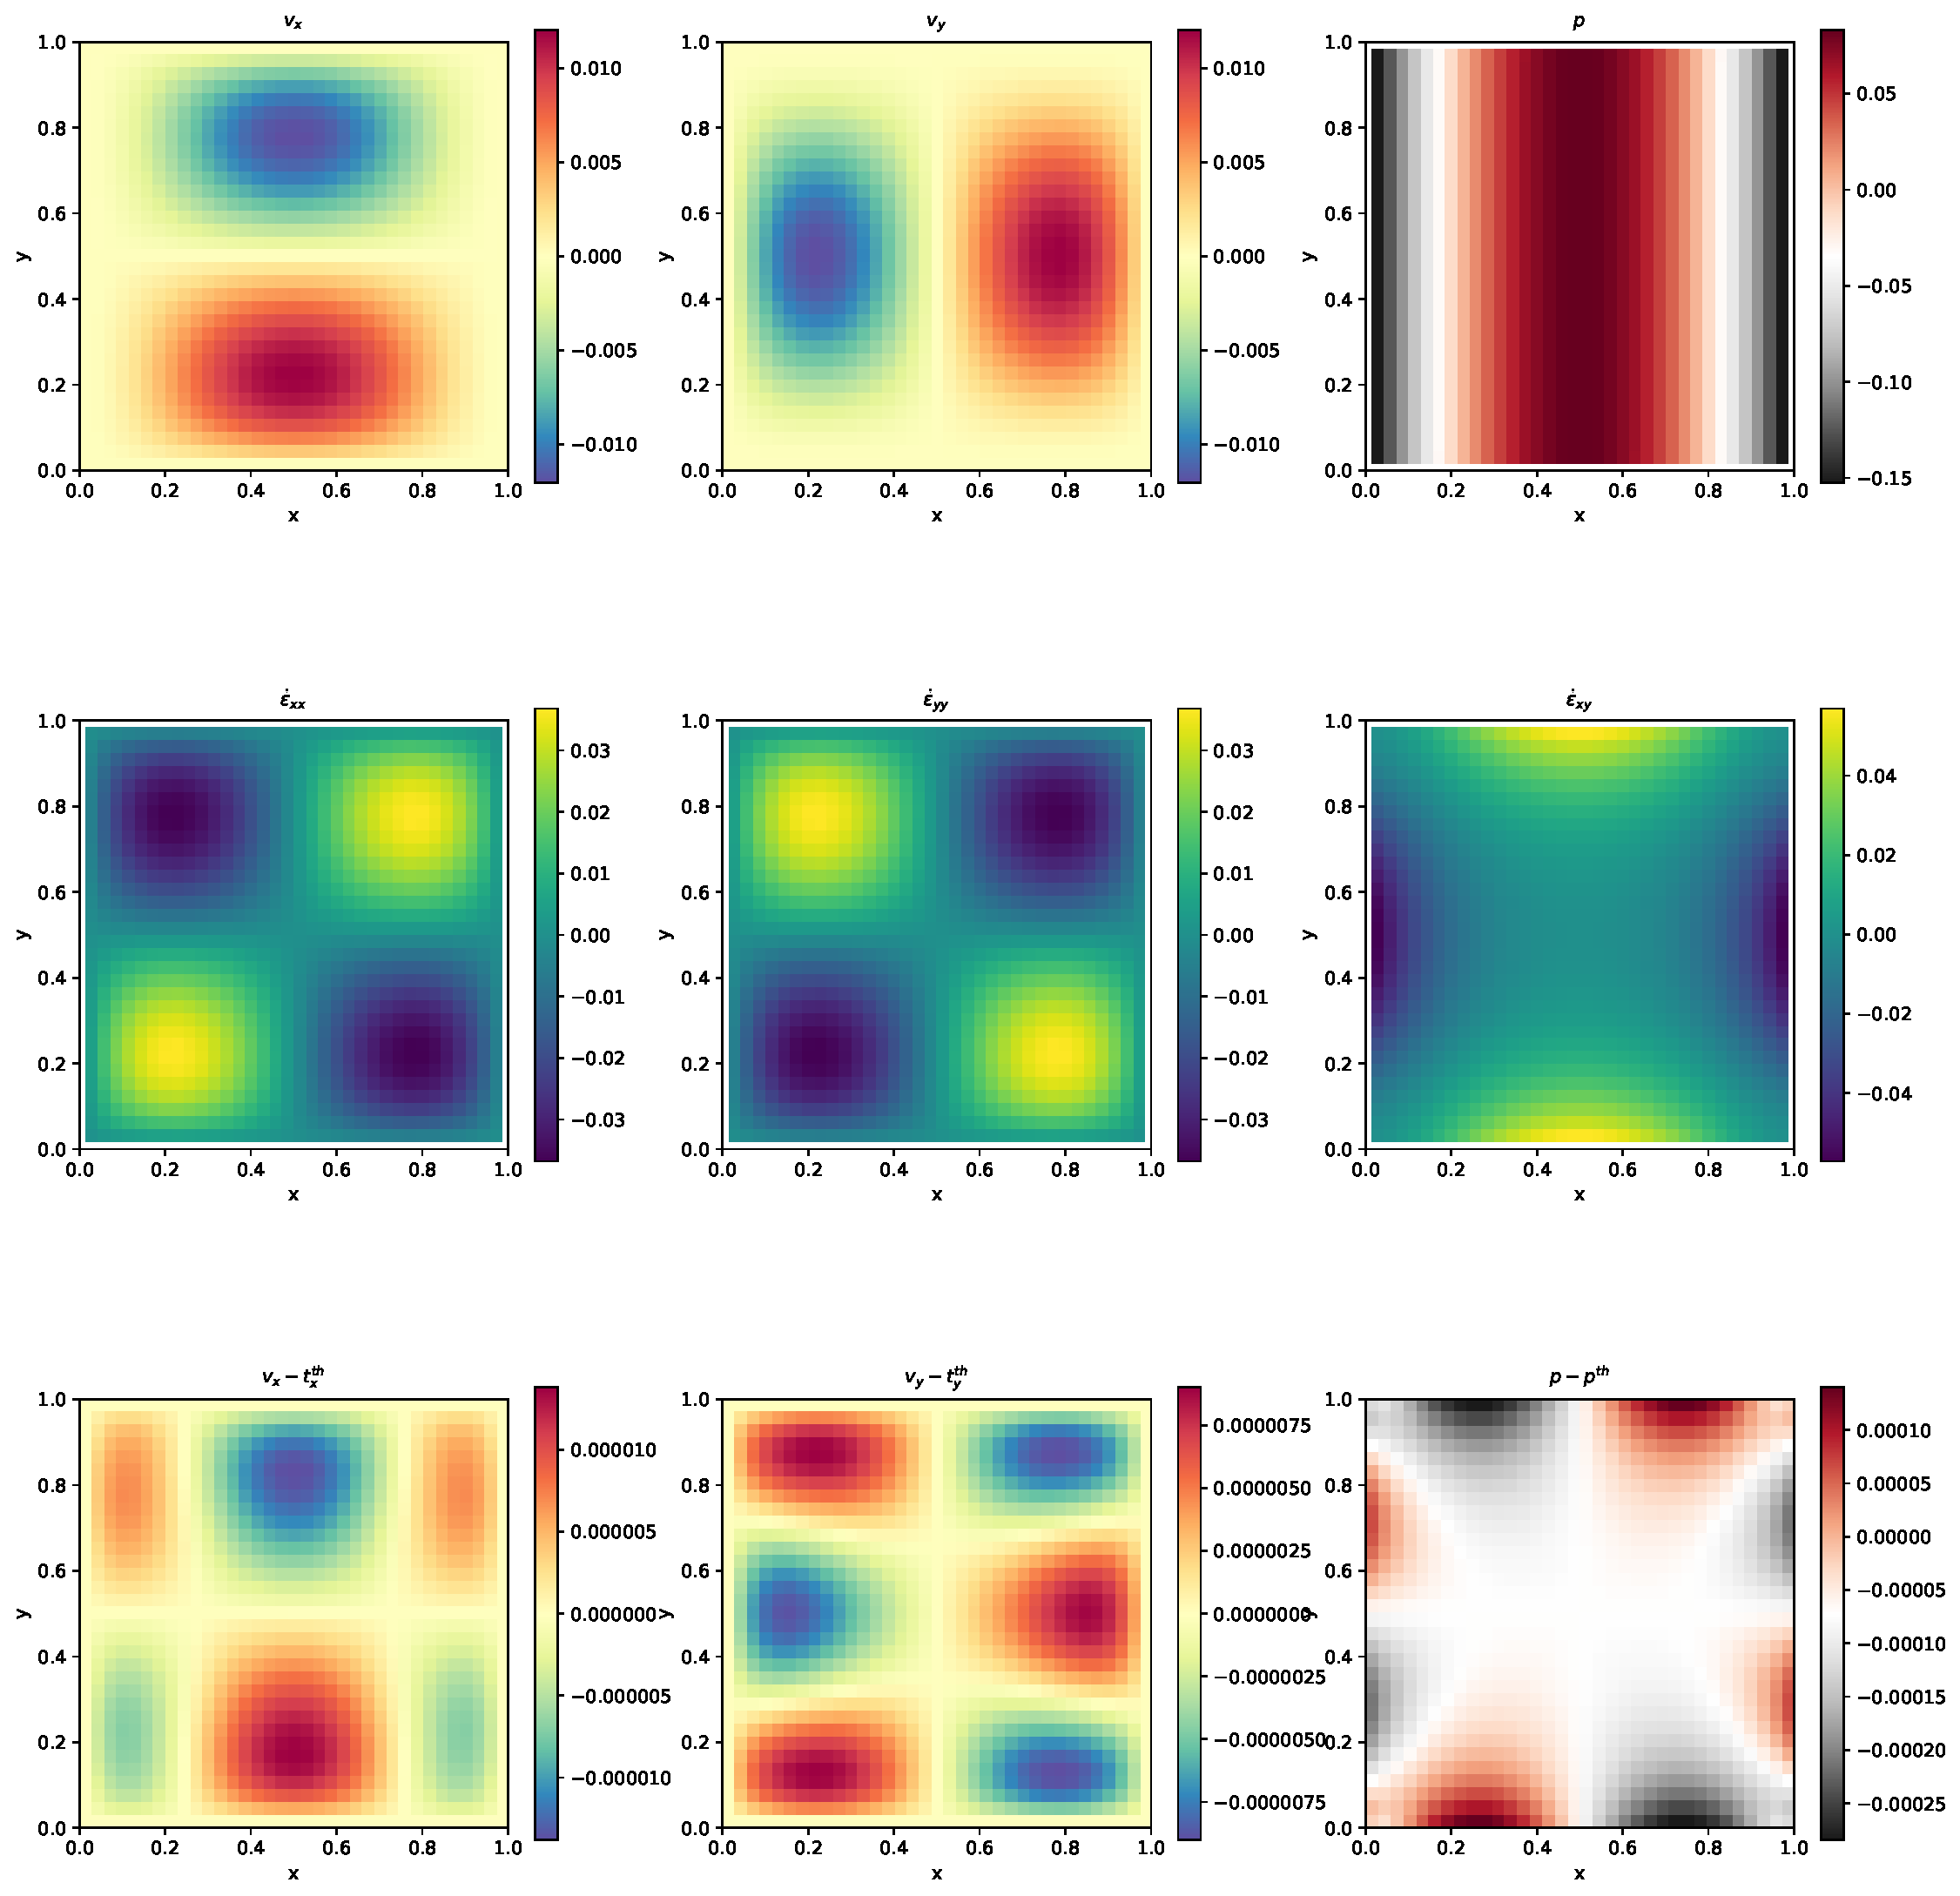
\includegraphics[width=16cm]{python_codes/fieldstone/solution.pdf}

\begin{center}
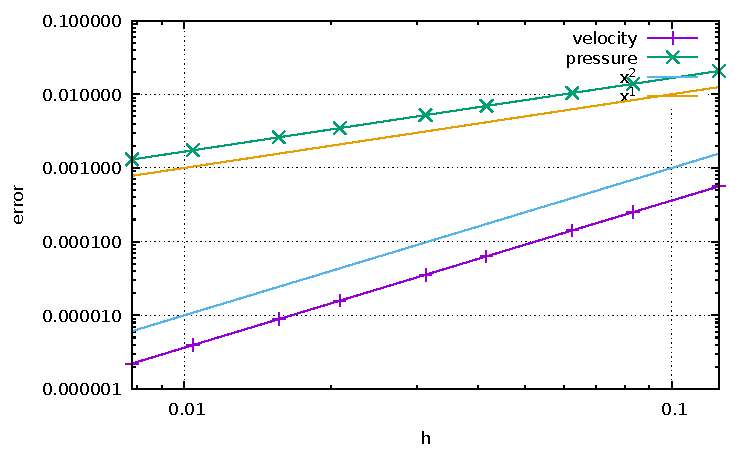
\includegraphics[width=12cm]{python_codes/fieldstone/errors.pdf}\\
Quadratic convergence for velocity error, 
linear convergence for pressure error, as expected.
\end{center}

ToDo:

pressure normalisation?

different cmat, a la schmalholz

To go further:
\begin{enumerate}
\item make your own analytical solution
\end{enumerate}
